\documentclass{article}
\usepackage{graphicx}
\usepackage[fontsize=11pt]{scrextend}
\title{PowerEnjoy Service - Design Document}
\begin{document}

	\section{ARCHITECTURAL DESIGN}
	
	\subsection{High level components and their interaction}
	\begin{figure}[h]
	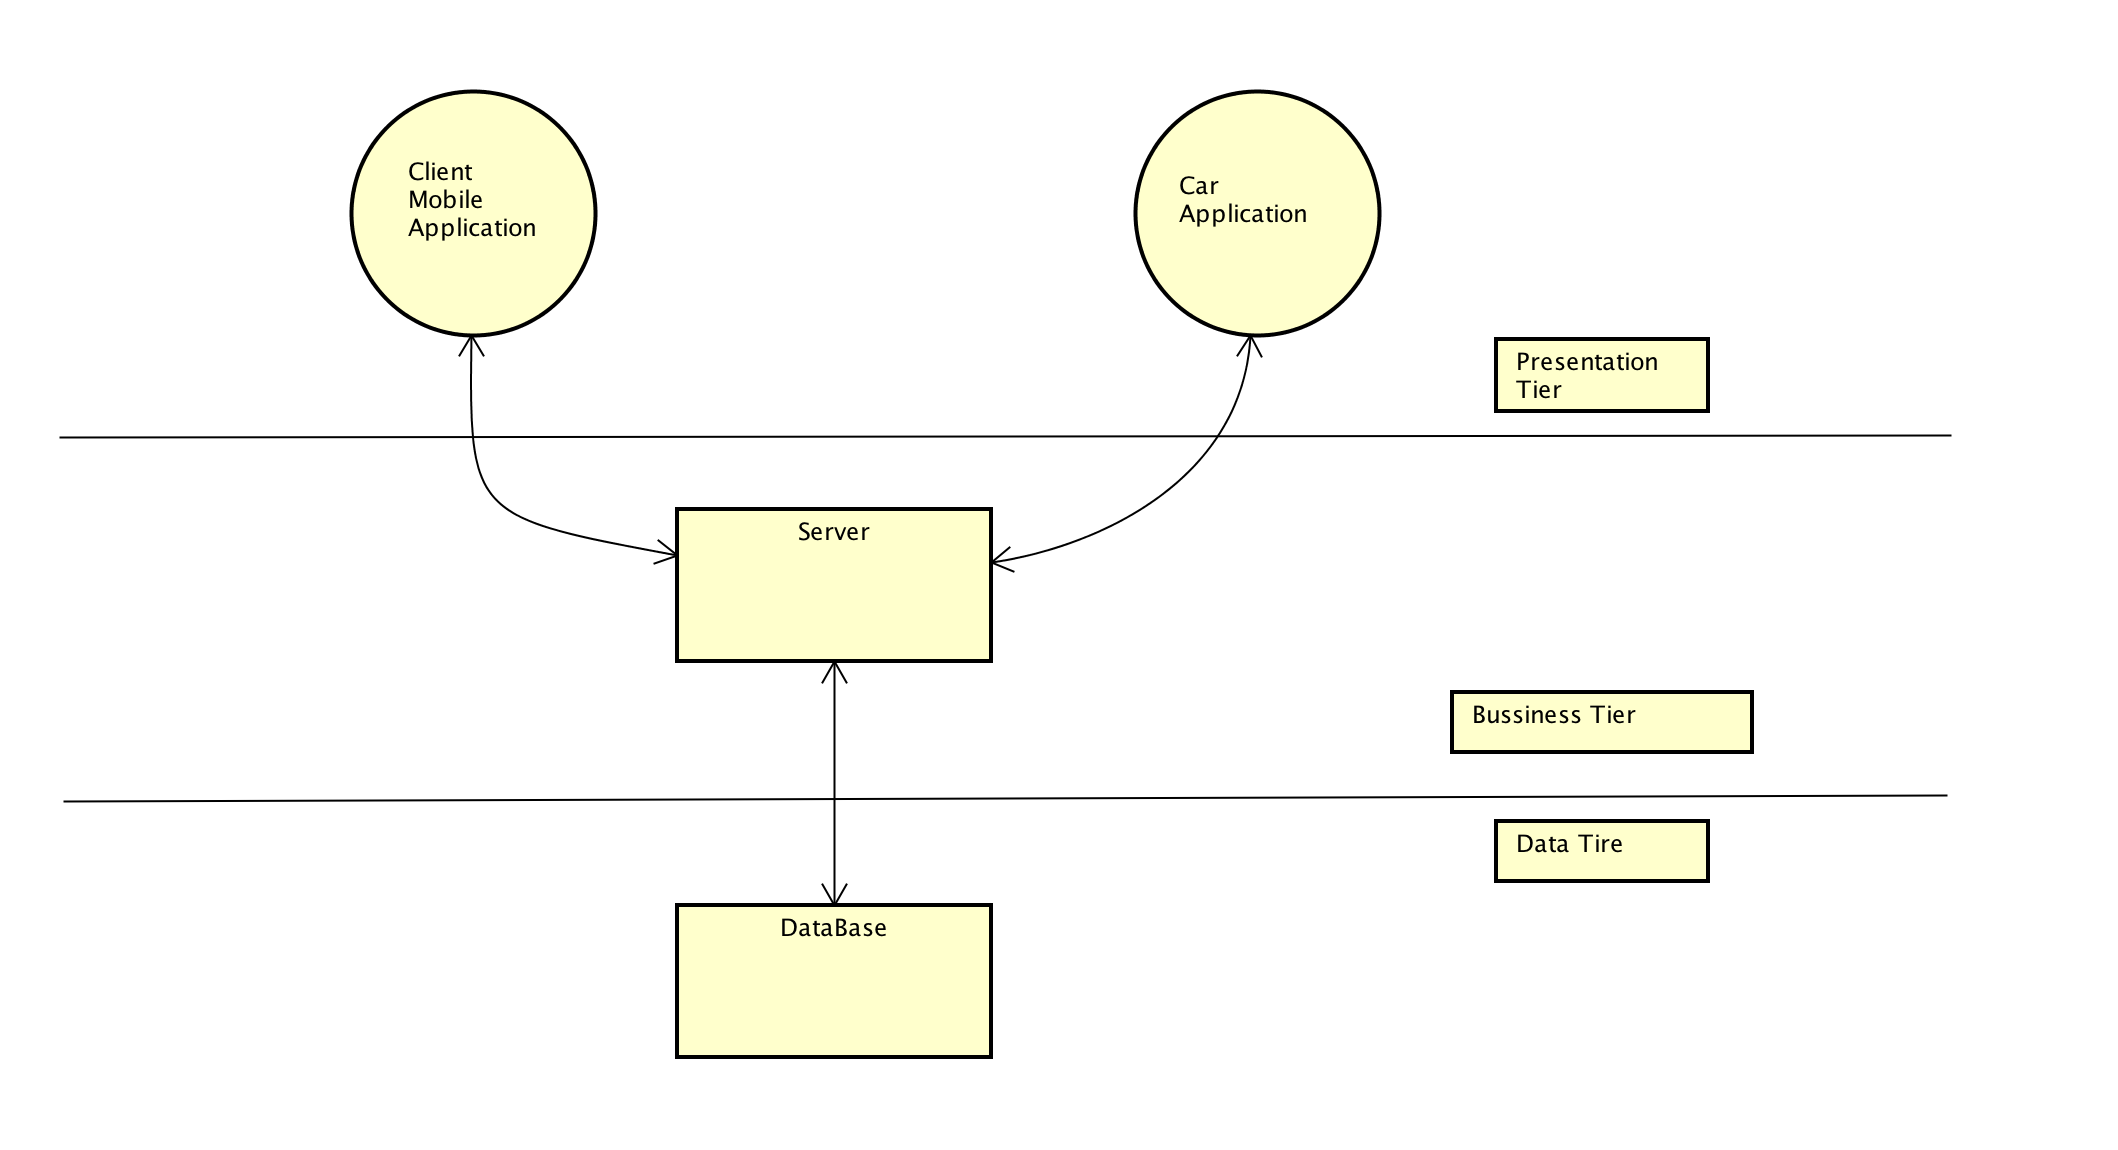
\includegraphics[width=\textwidth]{High_Level}
	\end{figure}
	Here we choose to use the 3 tier architacture: The Presentation tier including the Client Mobile Application and the Car Application; The Bussiness tier including the Server; The Data tire including the DataBase
	\newpage
	
	\subsection{Component view}
	\begin{figure}[h]
	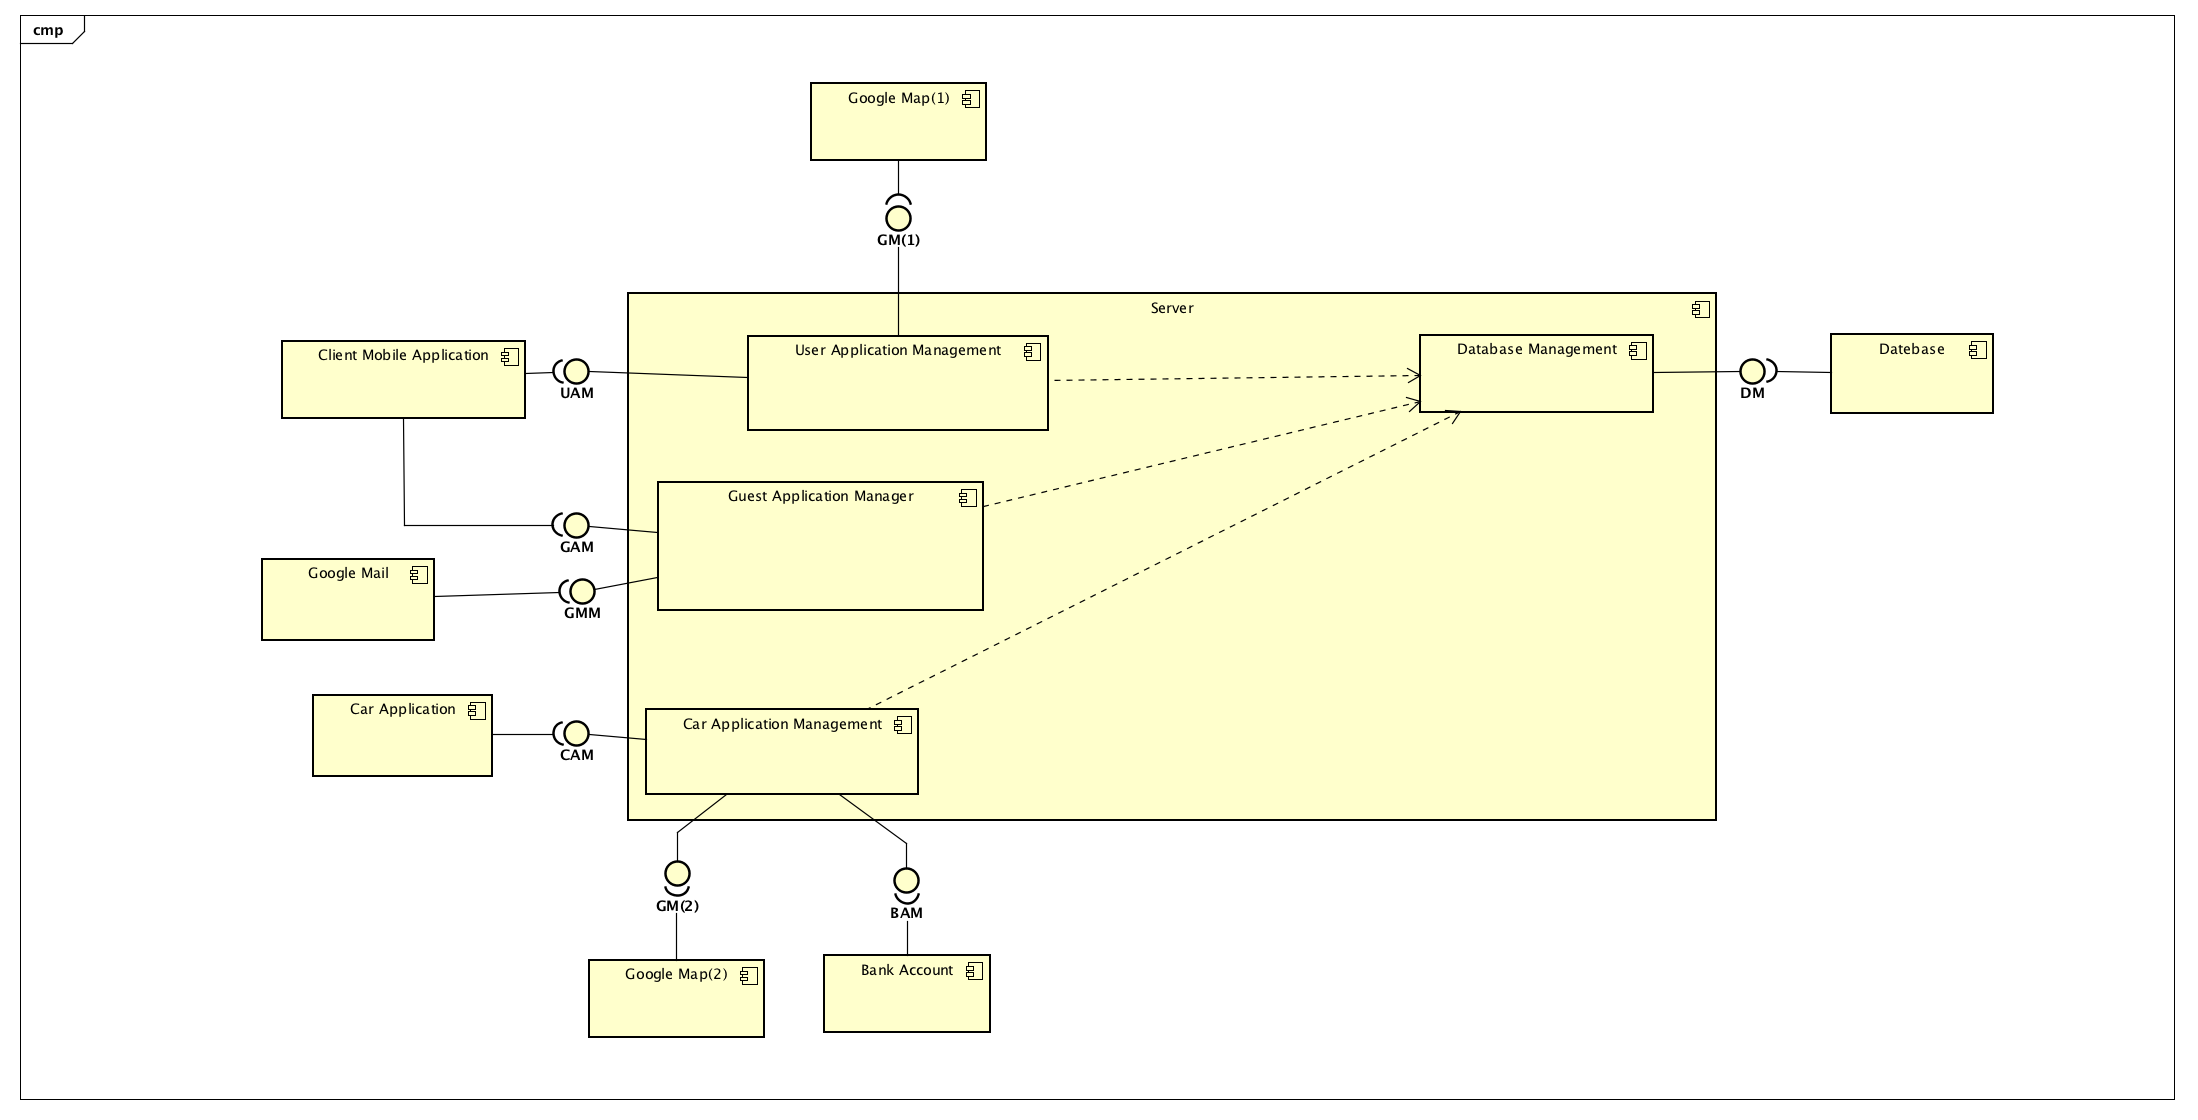
\includegraphics[width=\textwidth]{CV_Server}
	\end{figure}
	For the Server, there should be several interfaces, which are in charge of communicating with other components: 
	\begin{itemize}
		\item \textbf{User Application Manager} : Component that provides the interface for the users of the system and the Google Map. User Application Manager should provides the options of checking the available car around the specified position, reserving car and canceling the reservation. With the help of the Google Map, the system can know the location of the user.
		\item \textbf{Guest Application Manager} : Component that provides the interfaces for the unregistered guest of the system and the Google Mail. It provides the option to create an account. Finishing the register, the system would send an e-mail to the guest through the Google Mail.
		\item \textbf{Car Application Manager} : Component that provides the interface for the car Application, Google Map and Bank Account. The Car Application Manager can know the location of the car, charge the specified bank account and send the instruction to the car.
		\item \textbf{Database Manager} : Component that provides the interface for the Database for collecting the information which are collected by other components.   
	\end{itemize}
	\newpage
	\begin{figure}[h]
	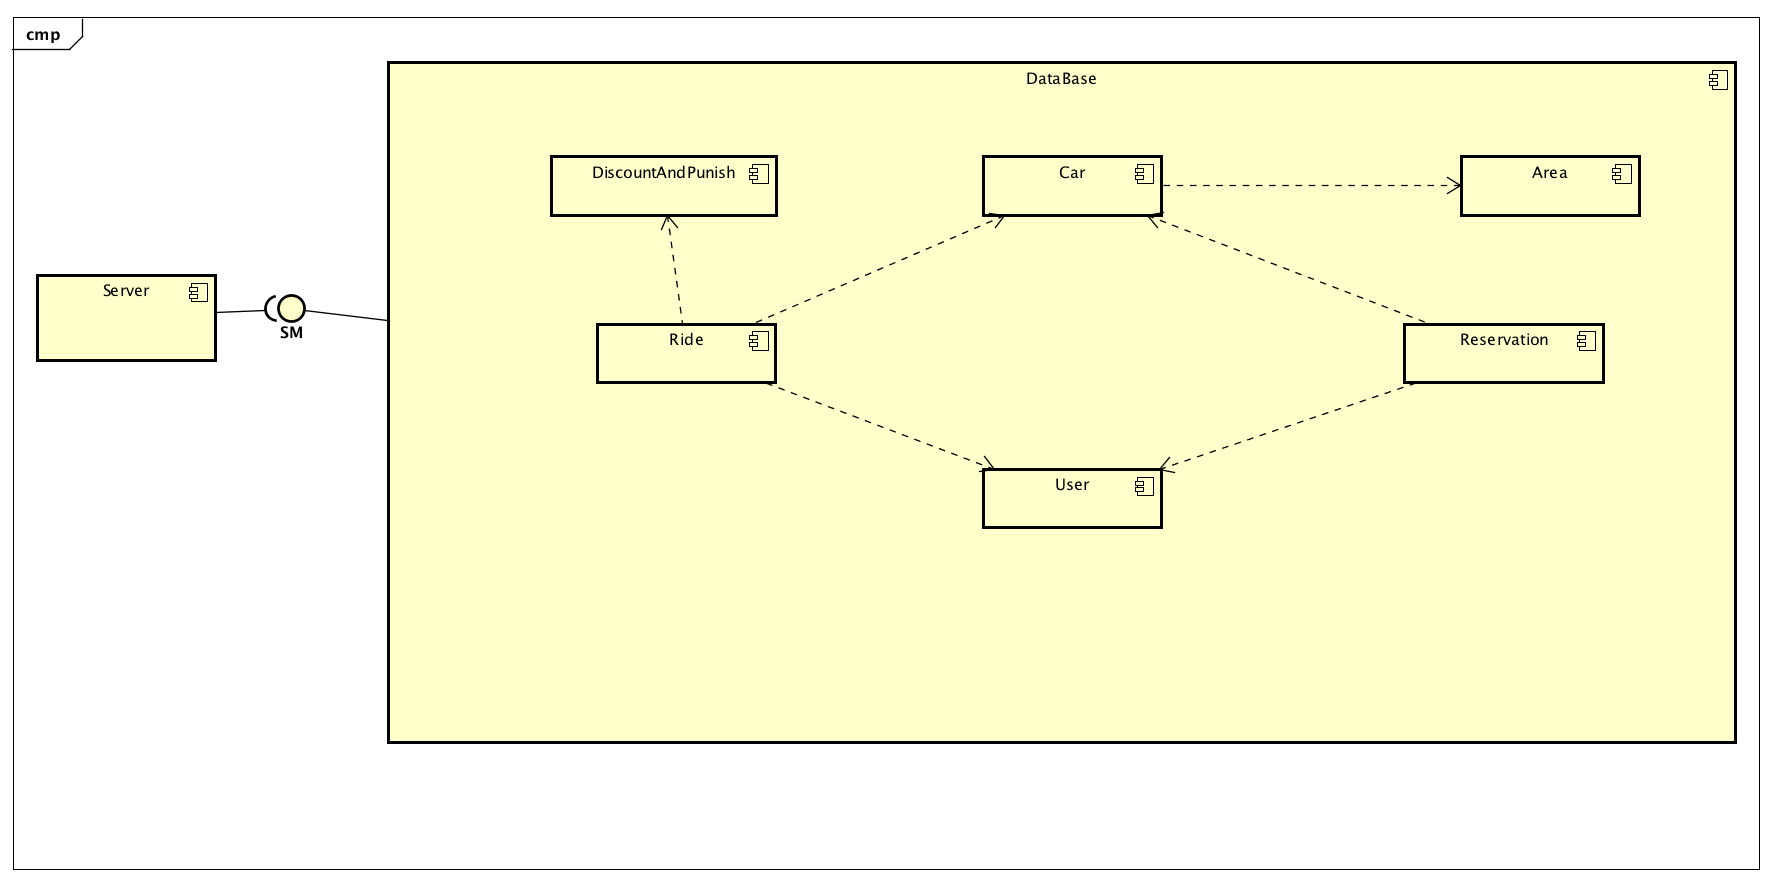
\includegraphics[width=\textwidth]{CV_Database}
	\end{figure}
	For the Database, there are several component for storing the data of the system. The Database should provides the interface of the Server for information exchange. Through the interface, the Server can transmit and  store the information in the Database. The Server can also retrieve the information from the Database according to the corresponding instruction.

	\begin{itemize}
		\item \textbf{Car} : Component that stores the information of the cars. The Car should stores the position, plate, battery, capacity, 	state and the currentPosition of each car.
		\item \textbf{User} : Component that stores the information of the users. The User should stores the credential and the paymentInfo of each user.
		\item \textbf{Ride} : Component that stores the information of the riding. The Ride should stores the riding information, including the renting car, corresponding user and so on.
		\item \textbf{Reservation} : Component that stores the information of the reservation. The Reservation should stores the user and the corresponding car of each reservation.
		\item \textbf{DiscountAndPunish} : Component that stores the information of the discount and punish of each ride. For each ride, when finishing the riding, the DiscountAndPunish component should provide the information about the discount and the punish, for calculating the total charging.
		\item \textbf{Area} : Component that stores the area of each position.
	\end{itemize}
	\newpage

	\section{Requirement traceability}
	In this section, we are going to show a precise list of all the functional requirements and their corresponding mapping to component in the architecture.(for more detailed view of how these components contact with others and the interfaces of these components, please refer to the high level architecture and the component interface)
	\begin{itemize}
		\item\textbf{[G1]}Users can register to the system and get the password by providing credentials and payment information
		\newline - Guest Application Manager
		\newline - Database Manager
		\newline - User
		
		\item\textbf{[G2]}Registerd users can log in by providing the correct credentials
		\newline - User Application Manager
		\newline - Database Manager
		\newline - User
		
		\item\textbf{[G3]}Registered users can find the locations of available cars within a certain distance from their current location or from a specified address
		\newline - User Application Manager
		\newline - Database Manager
		\newline - Car 
		\newline - Area
		
		\item\textbf{[G4]}Among the available cars in a certain geographical region, users must be able to reserve a single car for up to one hour before they pick it up.
		\newline - User Application Manager
		\newline - Database Manager
		\newline - User
		\newline - Car
		\newline - Reservation
		
		\item\textbf{[G5]}If a car is not picked‐up within one hour from the reservation, the system tags the car as available again, and the reservation expires; the user pays a fee of 1 EUR.
		\newline - Car
		\newline - Reservation
		\newline - Database Manager
		\newline - Car Application Manager
		
		\item\textbf{[G6]}A user that reaches a reserved car must be able to tell the system she’s nearby, so the system unlocks the car and the user may enter.
		\newline - User Application Manager
		\newline - Database Manager
		\newline - Reservation
		\newline - Car
		
		\item\textbf{[G7]}As soon as the engine ignites, the system starts charging the user for a given amount of money per minute; the user is notified of the current charges through a screen on the car.
		\newline - Car Application Manager
		\newline - Database Manager
		\newline - Ride
		\newline - Car
		
		\item\textbf{[G8]}The user is notified of the current charges through the screen on the car
		\newline - Car
		\newline - Ride
		\newline - Database
		\newline - Car Application Manager
				
		\item\textbf{[G9]}The system stops charging the user as soon as the car is parked in a safe area and the user exits the car; at this point, the system locks the car automatically.
		\newline - Car Application Manager 
		\newline - Database Manager
		\newline - Car
		\newline - Area
		
		\item\textbf{[G10]}The users can know the locations of the safe areas
		\newline - User Application Manager
		\newline - Database Manager
		\newline - Area
		
		\item\textbf{[G11]}If the system detects the user took at least two other passengers onto the car, the system applies a discount of 10\% on the last ride.
		\newline - Car Application Manger 
		\newline - Database Manager 
		\newline - Ride
		\newline - DiscountAndPunish
				
		\item\textbf{[G12]}If a car is left with no more than 50\% of the battery empty, the system applies a discount of 20\% on the last ride.
		\newline - Car Application Manger 
		\newline - Database Manager 
		\newline - Car
		\newline - Ride
		\newline - DiscountAndPunish
		
		\item\textbf{[G13]}If a car is left at special parking areas where they can be recharged and the user takes care of plugging the car into the power grid, the system applies a discount of 30\% on the last ride.
		\newline - Car Application Manger 
		\newline - Database Manager 
		\newline - Car
		\newline - Area
		\newline - Ride
		\newline - DiscountAndPunish
		
		\item\textbf{[G14]}If a car is left at more than 3 KM from the nearest power grid station or with more than 80\% of the battery empty, the system charges 30\% more on the last ride to compensate for the cost required to re-charge the car on-site.
		\newline - Car Application Manager
		\newline - Database Manager
		\newline - Car 
		\newline - Area
		\newline - Ride
		\newline - DiscountAndPunish
		
		\item\textbf{[G15]}If the user enables the money saving option, he/she can input his/her final destination and the system provides information about the station where to leave the car to get a discount. This station is determined to ensure a uniform distribution of cars in the city and depends both on the destination of the user and on the availability of power plugs at the selected station.
		\newline - User Application Manager
		\newline - Database Manager
		\newline - Car
		\newline - Area
		\newline - Reservation
		
		
		
	\end{itemize}

\end{document}